% [normalized] vector
\newcommand{\V}[1]{\ensuremath{\mathbf{#1}}}
\newcommand{\NV}[1]{\ensuremath{\mathbf{\hat{#1}}}}

\begin{frame}
\frametitle{Matice a prostory}
	\begin{itemize}
		\item Model je namodelovaný v tzn. model space prostoru
    \item Vrcholy modelu se po vynásobení modelovou maticí přesunou do world space prostoru - prostoru scény
    \item Celá scéna se poté transformuje pomocí view matice tak, aby to simulovalo pohled z kamery
    \item Následuje projekce do clip space pomocí projekční matice
    \item Výstup vertex shaderu by měl být v clip space
	\end{itemize}
  \begin{figure}[h]
    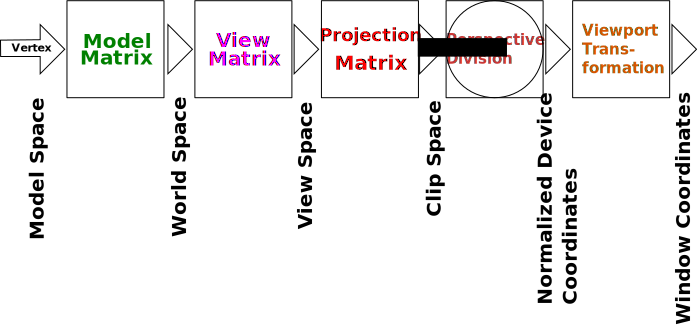
\includegraphics[width=10cm,keepaspectratio]{pics/linear/space.pdf}
  \end{figure}
\end{frame}


\begin{frame}
  \frametitle{Opakování Lingebry}
  Vektorový prostor
  \pause
  \begin{align*}
    \text{Vektory }\V{v}&(V,+,-) &
    \text{Skaláry }a&(S,+,-,*,{}^{-1})\\
    a(b\V{v}) &= (ab)\V{v} & 1\V{v} &= \V{v} \\
    a(\V{u}+\V{v}) &= a\V{u} + a\V{v} & (a+b)\V{v} &= a\V{v} + b\V{v}
  \end{align*}
  \pause
  Lineární kombinace
  \pause
  \begin{equation*}
    \V{v} = a_1\V{v}_1 + a_2\V{v}_2 + \dotsb + a_n\V{v}_n
  \end{equation*}
  \pause
  \begin{itemize}
    \item Lineární (ne)závislost
    \item Dimenze
    \item Báze
  \end{itemize}
\end{frame}

\begin{frame}
  \frametitle{Lineární transformace}
  $f$ zachovává lineární kombinaci :
  \begin{equation*}
    f(a_1\V{v}_1 + \dotsb + a_n\V{v}_n) = a_1f(\V{v}_1) + \dotsb + a_nf(\V{v}_n)
  \end{equation*}
  \pause
  Transformujeme $\V{v} = (x,y,z)^T$
  \begin{align*}
    \V{v} &= x\NV{x} + y\NV{y} + z\NV{z} & \NV{x} = (1,0,0)^T, \dotsc \\
    f(\V{v}) &= xf(\NV{x}) + yf(\NV{y}) + zf(\NV{z})
  \end{align*}
  (\NV{v} je normalizovaný vektor)
  \pause
  \begin{equation*}
    f(\V{v})_{x,y,z} = xf(\NV{x})_{x,y,z} + yf(\NV{y})_{x,y,z} + zf(\NV{z})_{x,y,z}
  \end{equation*}
  \pause
  \begin{align*}
    f(\V{v}) &= \begin{pmatrix}
    f(\NV{x})_x&f(\NV{y})_x&f(\NV{z})_x\\
    f(\NV{x})_y&f(\NV{y})_y&f(\NV{z})_y\\
    f(\NV{x})_z&f(\NV{y})_z&f(\NV{z})_z
  \end{pmatrix}\begin{pmatrix}x\\y\\z\end{pmatrix}
  \end{align*}
  \pause
  \begin{itemize}
    \item[\color{red}!!!] Transformujeme mezi bázemi. Aspoň jedna musí být zdokumentovaná.
  \end{itemize}
\end{frame}


\begin{frame}
    \frametitle{Měřítko - Scale}
    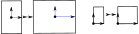
\includegraphics[width=\textwidth]{pics/linear/scale.pdf}
    \begin{align*}
        (1,0,0)&\rightarrow(x,0,0) & (0,1,0)&\rightarrow(0,y,0) & (0,0,1)&\rightarrow(0,0,z)
    \end{align*}
    \pause
    \begin{align*}
        S(x, y, z) &= \begin{pmatrix}
            x & 0 & 0 \\
            0 & y & 0 \\
            0 & 0 & z
        \end{pmatrix} \\
        S(x, y, z)^{-1} &= S(x^{-1}, y^{-1}, z^{-1}) \\
        \det S(x,y,z) &= xyz 
    \end{align*}
\end{frame}

\begin{frame}
    \frametitle{Rotace}

    Elementární rotace 
    \begin{align*}
        R_x(\alpha) &= \begin{pmatrix}
                1 & 0 & 0 \\
                0 & \cos \alpha & -\sin \alpha \\
                0 & \sin \alpha & \cos \alpha
            \end{pmatrix} &
        R_y(\alpha) &= \begin{pmatrix}
                \cos \alpha & 0 & \sin \alpha \\
                0 & 1 & 0 \\
                -\sin \alpha & 0 & \cos \alpha
            \end{pmatrix} \\
        R_z(\alpha) &= \begin{pmatrix}
                \cos \alpha & -\sin \alpha & 0 \\
                \sin \alpha & \cos \alpha & 0 \\
                0 & 0 & 1
            \end{pmatrix}
    \end{align*}

    \vfill

    Eulerovy úhly $\alpha, \beta, \gamma$
    \begin{equation*}
        R_x(\alpha)R_y(\beta)R_z(\gamma) \ne R_z(\gamma)R_y(\beta)R_x(\alpha)
    \end{equation*}
    \begin{itemize}
        \item[\color{red}:(] Nepraktické, neintuitivní, moc kombinací.
        \item[\color{red}:(] První otočení otáčí další osy $\rightarrow$ špatně se skládají.
    \end{itemize}
\end{frame}

\begin{frame}
    \frametitle{Lepší reprezentace rotací}

    Osa rotace $\NV{e} = (x,y,z)$ a úhel $\theta$
    \begin{align*}
        R((x,y,z), \theta) = \begin{pmatrix}
            x^2(1-c) + c & xy(1-c) - zs & xz(1-c) + ys \\
            yx(1-c) + zs & y^2(1-c) + c & yz(1-c) + xs \\
            zx(1-c) - ys & zy(1-c) + xs & z^2(1-c) + c \end{pmatrix} \\
        c = \cos\theta, s = \sin\theta
    \end{align*}
    \vfill
    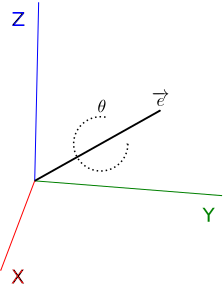
\includegraphics[height=.5\textheight]{pics/linear/axis-angle.pdf}
    \vfill
    Rodriguezův vzorec :
    \begin{equation*}
        \V{v}' = c\V{v} + s(\NV{e}\times\V{v}) + \NV{e}(\NV{e}\cdot\V{v})(1-c)
    \end{equation*}
\end{frame}

\begin{frame}
    \frametitle{Vlastnosti}
    Special Orthogonal Group $SO(3)$
    \begin{align*}
        \det R(\V{e}, \theta) &= 1 & {\color{blue}?} \\
        R(\V{e}, \theta)^{-1} &= R(\V{e}, \theta)^T = R(\V{e}, -\theta) \\
        R(\V{e}_1,\theta_1)\dotsm R(\V{e}_n,\theta_n) &= R(\dotso)
    \end{align*}
    \pause\vfill
    Orthogonal Group $O(3)$
    \begin{align*}
        \det F(\dotso) &= \pm1 & {\color{blue}?}
    \end{align*}
    \pause\vfill
    \begin{itemize}
        \item[\color{green}:)] Rotace + "Scale" = Zrcadlení
    \end{itemize}
    \begin{equation*}
        M(\NV{e}) = S(-1)R(\NV{e}, \pi)
    \end{equation*}
\end{frame}

\begin{frame}
    \frametitle{Posun}
    \begin{equation*}
        T(x,y,z) = \begin{pmatrix}
            1&0&0&x\\0&1&0&y\\0&0&1&z\\0&0&0&1
        \end{pmatrix}
    \end{equation*}
    \vfill
    \begin{equation*}
        T(\V{v})^{-1} = T(-\V{v})
    \end{equation*}
    \vfill
    \begin{itemize}
        \item Spolu s $SO(3)$ tvoří \textbf{Proper Rigid Transform}.
        \item Spolu s $O(3)$ tvoří \textbf{Rigid Transform}.
        \item Transformace pevného tìlesa.
    \end{itemize}
\end{frame}


\begin{frame}
    \frametitle{Skládání transformací}
    Asociativita
    \begin{equation*}
        F_1F_2\dotsb F_n\V{x} = (F_1F_2\dotsb F_n)\V{x}
    \end{equation*}
    \begin{itemize}
        \item Ve VS násobím jedinou maticí.
        \item Matice skládám při průchodu scénou.
    \end{itemize}
    \pause\vfill
    Inverzní transformace
    \begin{equation*}
        (F_1F_2\dotsb F_n)^{-1} = F_n^{-1}\dotsb F_2^{-1}F_1^{-1}
    \end{equation*}
    \begin{itemize}
        \item Při průchodu se dá složit i inverzní matice.
    \end{itemize}
\end{frame}

\begin{frame}
    \frametitle{Vyjádření maticí $4\times4$}
    \begin{itemize}
        \item Vektor $(x,y,z)^T \rightarrow (x,y,z,0)^T$
        \item Bod $(x,y,z)^T \rightarrow (x,y,z,1)^T$
        \item[\color{red}!!!] Tohle nejsou homogenní souřadnice!
    \end{itemize}
    \pause
    \begin{align*}
        \begin{pmatrix}
            F & \V{t} \\
            \V{0}^T & 1
        \end{pmatrix}\begin{pmatrix}\V{v}\\w\end{pmatrix}
        &= \begin{pmatrix}
            F\V{v} + {\color{blue}\V{t}w} \\
            \V{0}^T\V{v} + {\color{blue}1w}
        \end{pmatrix} \\
        \begin{pmatrix}
            3\times3 & 3\times1 \\
            1\times3 & 1\times1
        \end{pmatrix}\begin{pmatrix}3\times1\\1\times1\end{pmatrix}
        &= \begin{pmatrix}
            3\times3 \cdot 3\times1 + 3\times1 \cdot 1\times1 \\
            1\times3 \cdot 3\times1 + 1\times1 \cdot 1\times1
        \end{pmatrix}
    \end{align*}
    \pause\vfill
    Kombinace bodů a vektorů :
    \begin{align*}
        V + V &= V & 0+0 &= 0 \\
        P - P &= V & 1-1 &= 0 \\
        P \pm V &= P & 1\pm 0 &= 1 \\
        P + P &= \color{red}??? & 1+1 &= 2
    \end{align*}
\end{frame}



\begin{frame}
    \frametitle{Skládání}
    \begin{equation*}
        \begin{pmatrix}
            F_1 & \V{t}_1 \\
            \V{0}^T & 1
        \end{pmatrix}
        \begin{pmatrix}
            F_2 & \V{t}_2 \\
            \V{0}^T & 1
        \end{pmatrix}\V{p}
        = \begin{pmatrix}
            F_1F_2 + \V{t}_1\V{0}^T & F_1\V{t}_2 + \V{t}_11 \\
            \V{0}^TF_2 + 1\V{0}^T & \V{0}^T\V{t}_1 + 1\cdot1
        \end{pmatrix}\V{p}
    \end{equation*}
    \pause
    \begin{equation*}
        \begin{pmatrix}
            F_1F_2 & F_1\V{t}_2 + \V{t}_1 \\
            \V{0}^T & 1
        \end{pmatrix}
    \end{equation*}
    \pause\vfill
    Napřed $F$ a pak $T(\V{t})$ :
    \begin{equation*}
        \begin{pmatrix}
            F & \V{t} \\
            \V{0}^T & 1
        \end{pmatrix}
        =\begin{pmatrix}
            I & \V{t} \\
            \V{0}^T & 1
        \end{pmatrix}
        \begin{pmatrix}
            F & \V{0} \\
            \V{0}^T & 1
        \end{pmatrix}
    \end{equation*}
    \pause\vfill
    \begin{align*}
        (T(\V{t})F)^{-1} &= F^{-1}T(-\V{v}) \\
        \begin{pmatrix}
            F & \V{t} \\
            \V{0}^T & 1
        \end{pmatrix}^{-1}
        &= \begin{pmatrix}
            F^{-1} & -F^{-1}\V{t} \\
            \V{0}^T & 1
        \end{pmatrix}
    \end{align*}
\end{frame}

\begin{frame}
    \frametitle{Homogenní souřadnice}
    $\mathbf{RP}^N = \mathbb{R}^{N+1} \setminus \{\V{0}\}$ :
    \begin{itemize}
        \item N+1 souřadnic pro N-rozměrný prostor.
        \item[\color{red}!] Všechno jsou body.
        \item[\color{red}!] Ve 3D $(x, y, z, w)^T$ s aspoň jedním nenulovým prvkem.
        \item[\color{red}!] Každý bod má nekonečně mnoho reprezentací ($\V{p} \equiv k*\V{p}, k \in \mathbb{R} \setminus \{0\}$).
    \end{itemize}
    \pause\vfill
    $(x,y,z,0)$ jsou \textbf{ideální body} ležící v nekonečnu
    \begin{itemize}
        \item Leží ve směru vektoru $(x,y,z)$
        \item[\color{red}!!!] A zároveň i opačným směrem ($\V{p} \equiv -1\V{p}$)
        \item[\color{red}!!!] Nejsou to vektory, ty tu už nemáme.
    \end{itemize}
\end{frame}

\begin{frame}
    \frametitle{Projektivní prostor}
    \begin{itemize}
        \item Každý bod v $\mathbb{R}^3$ je přímka skrz počátek v $\mathbb{R}^4$.
        \item $k\V{p}$ je pohyb po té přímce.
        \item Počátkem procházejí všechny přímky, proto jsme ho odstranili.
        \item Perspektivní dělení počítá průsečík s rovinou $w = 1$.
    \end{itemize}
    \pause\vfill
    Projektivní rovina $\mathbf{RP}^2$
    \begin{itemize}
        \item Body $(x,y,z)$ bez $(0,0,0)$.
        \item Perspektivní dělení $(x,y,z) \rightarrow (x/z,y/z)$ promítá na rovinu $z=1$.
    \end{itemize}
\end{frame}
